\documentclass[preprint,3p,twocolumn]{elsarticle}

\usepackage{lineno}
\usepackage[draft]{hyperref}
%\modulolinenumbers[5]

\journal{Fusion Engineering and Design}
\bibliographystyle{elsarticle-num}
%%%%%%%%%%%%%%%%%%%%%%%

\begin{document}

\begin{frontmatter}

\title{Ion Cyclotron and Lower Hybrid Frequency Range Cold Magnetized Plasma Modelling in {ANSYS} {HFSS}}
%% Group authors per affiliation:
\author[IRFM]{Julien Hillairet\corref{mycorrespondingauthor}}
\author[ERM]{Riccardo Ragona}
\author[IRFM]{Laurent Colas}
\author[IRFM]{Walid Helou}
\author[ANSYS]{Frédéric Bocquet}

\cortext[mycorrespondingauthor]{Corresponding author}
\ead{julien.hillairet@cea.fr}
%% Authors affiliations
\address[IRFM]{CEA, IRFM, F-13108 Saint Paul-lez-Durance, France}
\address[ERM]{Laboratory for Plasma Physics, Royal Military Academy, (LPP-ERM/KMS), BE-1000, Brussels, Belgium}
\address[ANSYS]{ANSYS France}

\begin{abstract}
The coupling between cold magnetized plasmas with Ion Cyclotron and Lower Hybrid Resonance Frequency antennas is generally addressed using specifically developed codes. These antenna coupling codes often approximate the plasma to surface impedances described by 1D half infinite models. Depending of the mathematical approaches used by these codes, the modelled antennas can be described either in simplified 2D dimensions or in 3D complex geometries converted from CAD models. Such approaches add an additional step of model approximation/conversion which does not allow one to work directly on realistic antenna model and to rapidly assess the impact of geometry changes. Moreover, during the design phase, it is convenient to use the RF simulation to directly estimate the thermal and mechanical loads in the same software suite. The coupling calculation of both Ion Cyclotron and Lower Hybrid Resonance Frequency antennas is explored in this paper with ANSYS HFSS. The results obtained are compared with the fast coupling codes ALOHA and ANTITER II on both homogeneous and inhomogeneous cold magnetized plasmas. Good agreements are obtained when the boundary conditions in the full-wave modelling are properly setup. Advices are given in order to define correctly these boundary conditions and insure correct results.
\end{abstract}

\begin{keyword}
ICRH \sep Cold Plasma \sep Finite Elements
%\MSC[2010] 00-01\sep  99-00
\end{keyword}

\end{frontmatter}

\linenumbers

\section{Introduction}
Achieving the plasma temperature expected for nuclear fusion requires external heating systems, such as dedicated Radio-Frequency antennas. Dimensions, power level and manufacturing cost which are at stake make it impossible to build scale-one mock-up during design and prototyping phases. For that reason, modelling the electromagnetic interactions between magnetized plasmas and Radio-Frequency antennas is mandatory for nuclear fusion research. In this paper, we focus only on the RF coupling performances of these antenna to the tokamak edge plasma and not into the wave absorption mechanisms inside the plasma. 

During the last two decades, the availability of RF full wave software eased the design of Ion Cyclotron ({ICRF}) and Lower Hybrid Resonance Frequency systems ({LHRF}). As the both software and hardware progressed, the modelling of always more realistic and bigger components became possible, reducing the gap between CAD and RF models and accelerating the necessary feedback between mechanical and RF engineers. Nowadays, thermal or mechanical loads can be provided directly from the results of RF simulations inside integrated workflows, which make the design phase faster.

However, antenna to plasma coupling modelling with such tools was not possible unless some simplifications. Indeed, full wave codes didn't support since recently anisotropic and non homogeneous dielectric media. Plasma facing the antennas can be described in the cold-plasma approximation by the following relative permittivity tensor in the $e^{j\omega t}$ time-harmonic convention:
\begin{equation}
\varepsilon_r 
=
\left(
\begin{array}{ccc}
S & -jD & 0 \\
jD & S & 0 \\
0 & 0 & P
\end{array}
\right)
\end{equation}
where the parameters $S$, $D$, $P$ are described in \cite{Stix1992} and depends of the RF frequency, the plasma particle densities and the confining magnetic field. 

This is the reason why community codes such as {ANTITER II} \cite{Messiaen2011} or {TOPICA} \cite{Lancellotti2006} for {ICRF} and {TOPLHA} \cite{Milanesio2012}, {OLGA} \cite{Preinhaelter2017} or {ALOHA} \cite{Hillairet2010a} for LHRF, were developed specifically for that purpose. While these tools are generally faster than full-wave modelling, they mostly assume slab plasma and simplified antenna geometries to keep an analytical formulation of the problem. When dealing with detailled and curved antennas, poloidal and toroidal plasma curvatures, 3D numerical approaches are essential.  

Regarding coupling performances only, using constant dielectric for the fast-wave antenna loading is a good workaround to approximate the ICRF plasma coupling \cite{Messiaen2011a}. Such loads, using high permittivity medium such as (salty) water\cite{Messiaen2005} or BaTiO3 solutions\cite{Helou2018} are used in laboratory experiments. As a recent illustration, antenna coupling performances have been investigated substituting the plasma load  with a salty water tank in ANSYS HFSS \cite{Ravera2012, Qin2015} or with BaTiO3 in Microwave CST \cite{Bottollier-Curtet2011}. However, these solutions can't reproduce neither the inhomogeneity produced by increasing density in operational conditions or the medium gyrotropy and anisotropy effects on antenna loading. If these effect are not crucial for coupling calculations, they are for interest for other codes using antenna coupling quantities as input. As an example, the radiated spectrum generated by the antenna, which depend of the wavenumber in toroidal $k_z$ and poloidal $k_y$ directions, is an even function of $k_z$ but not of $k_y$ due to gyrotropy.

Since the last decade, full wave codes such as {COMSOL}, Microwave {CST} or {ANSYS} {HFSS} for example, have been able to define propagating medium as anisotropic tensor with eventually negative permittivity, spatial and frequency dependences. This ability allowed coupling\cite{Meneghini2009g, Shiraiwa2009} and absorption\cite{Meneghini2009} calculations of the C-Mod LH launcher. Recently, the open-source initiative \cite{Shiraiwa2017} allows modelling RF waves propagation in SOL plasmas. However, in all cases, a difficulty arises in the model setup concerning the boundary conditions at the edges of the cold plasma domain. Indeed, default radiation or absorbing boundary conditions such as Perfectly Matched Layer (PML) shipped in all these softwares are not designed to be used directly on the anisotropic material boundaries but instead on isotropic mediums. For antenna to plasma coupling, the plasma medium in which the antenna radiate is at the contrary considered as an semi-infinite medium and should be thus defined with attached ideal absorbing boundary conditions. 

Specific PML for anisotropic materials such as a magnetized cold plasma have been used in \cite{Jacquot2013b} and mathematically studied in  \cite{Becache2016, Becache2018}. Recently in \cite{Louche2017}, a 1D cold plasma has been modelled in CST Microwave Studio and compared against analytical solutions. Due to a software limitation to define non-homogeneous medium, a stratified PML has been used to mimic the single pass absorption in a bulk plasma. To obtain a precise solution, a large number of layers are required in the PML. 

Thanks to the collaboration between CEA, ITER and ANSYS, the RF modelling software ANSYS HFSS supports non-homogeneous anisotropic medium since 2016 (TBC). The purpose of this work is not to create a rigorous approach of the coupling simulation, to model the wave absorption mechanism in the plasma or to model non-linear effects such as sheaths creations on the antenna boundaries. The motivation is instead to assess the ability of HFSS to describe the usual range of experimental magnetized cold plasma parameters facing these antennas, away from resonances, in order to guide the RF designer during the design phase of an antenna. 


\section{LHCD Coupling}
In the Lower Hybrid Current Drive range of frequencies (2-6 GHz) and edge plasma densities in current tokamak experiments ($10^{17}-10^{18}$ $m^{-3}$), the cold plasma dielectric tensor is mostly diagonal and the form:
\begin{equation}
\varepsilon_r 
=
\left(
\begin{array}{ccc}
1 & 0 & 0 \\
0 & 1 & 0 \\
0 & 0 & P
\end{array}
\right)
\end{equation}
with $P\approx 1 - \frac{\omega_{pe}}{\omega}$ where $\omega_{pe}$ and $\omega$ are respectively the plasma and the RF angular frequency .  

\begin{figure*}
	\centering
	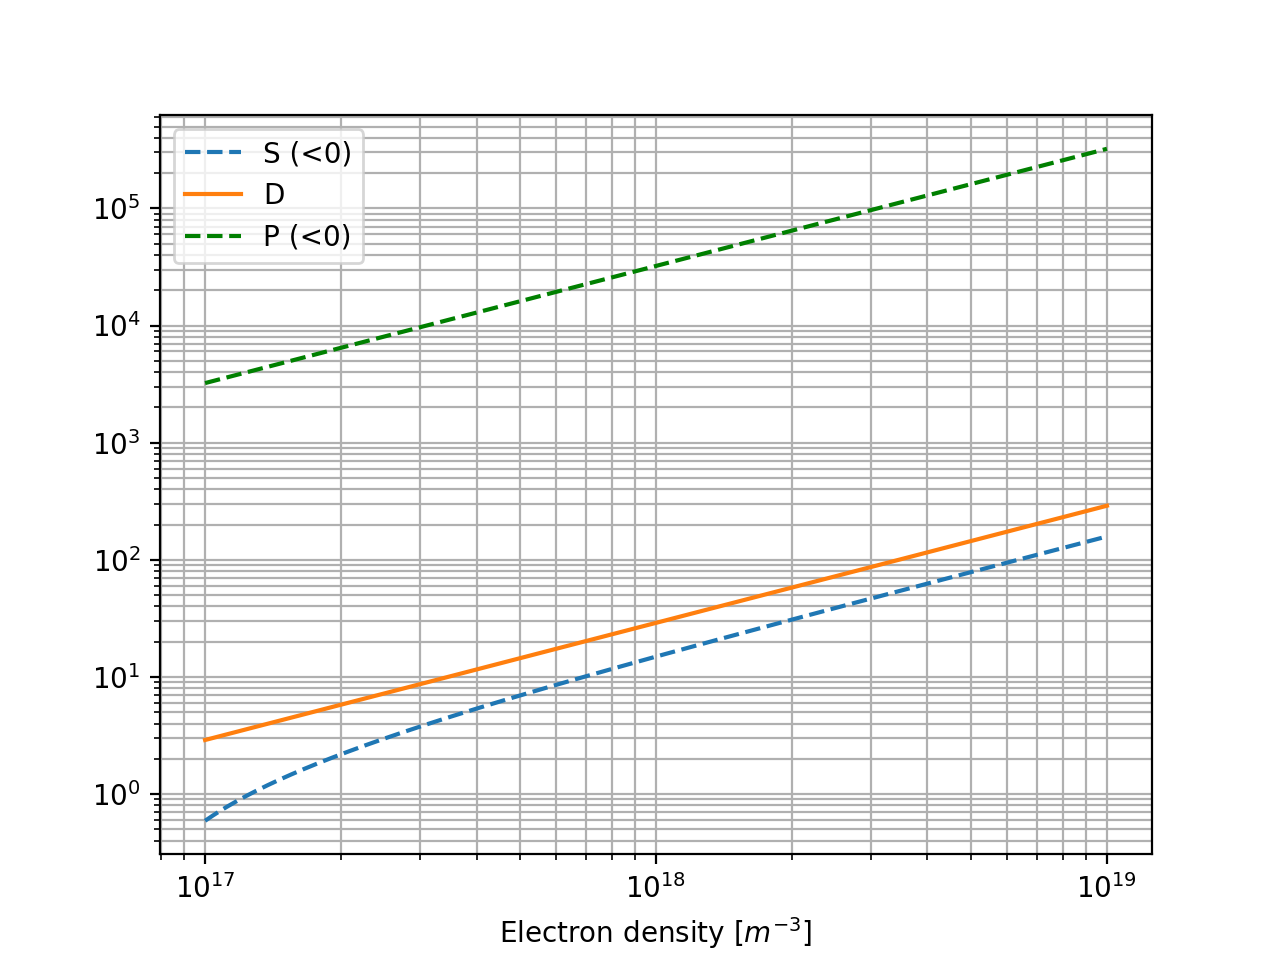
\includegraphics[width=0.48\linewidth]{figures/IC_SDP}
	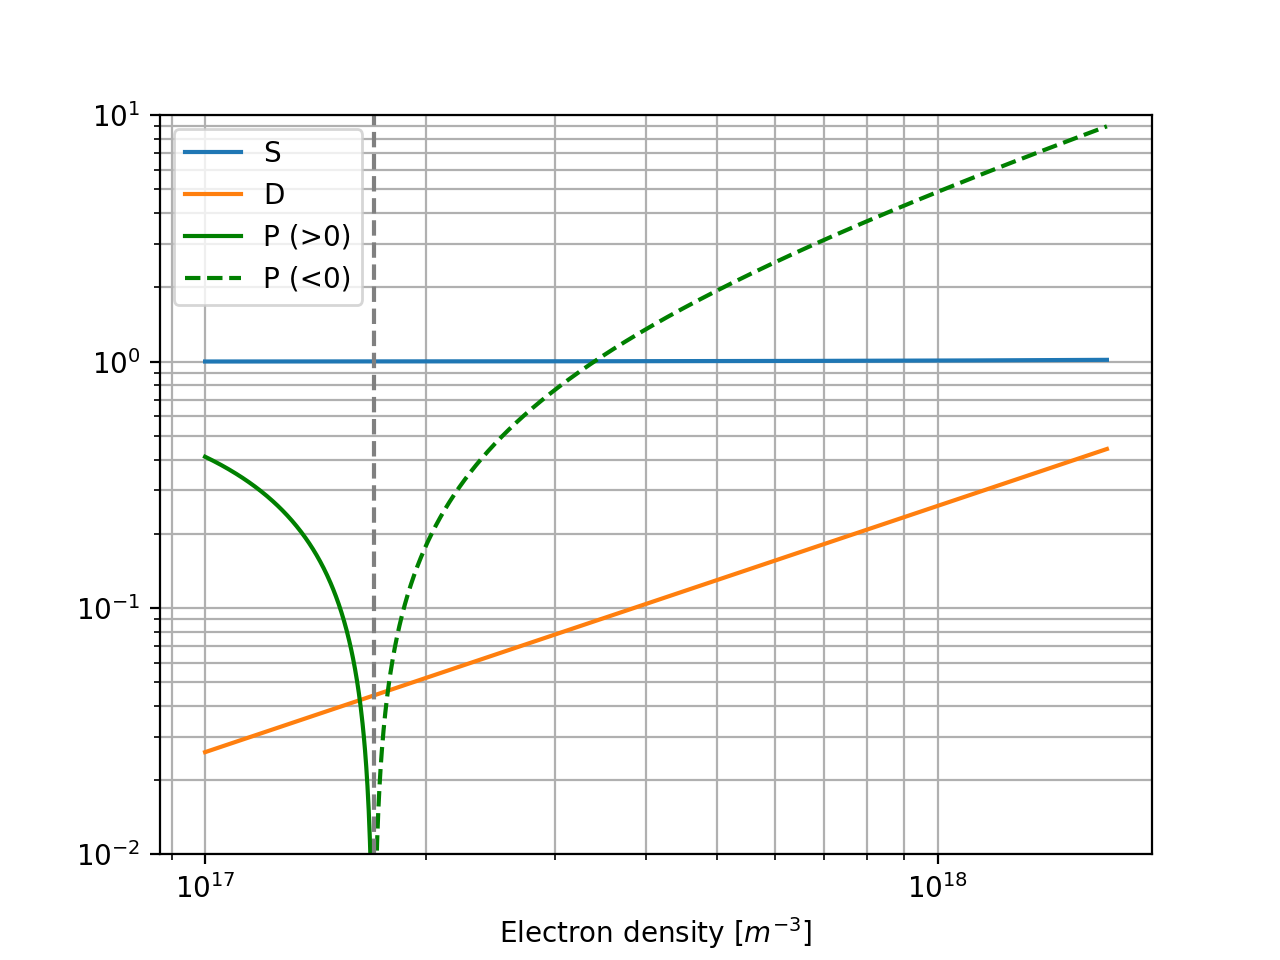
\includegraphics[width=0.48\linewidth]{figures/LH_SDP}
	\caption{Typical magnitudes of the relative permittivity tensor elements of a tokamak cold magnetized plasma for IC (left) and LH (right) range of parameters.}
	\label{fig:sdp_vs_density}
\end{figure*}


Depending the geometry considered, workarounds consist in adding progressively artificial losses (also know as "adiabatic absorbers") in order to attenuate the waves before they reach the propagation domain edges\cite{Oskooi2008} or to use symmetry boundary conditions to model axis-symmetric geometries REF??.   



\section{ICRH Coupling}
A simplified ICRH antenna model is compared with the coupling code ANTITER II  \cite{Messiaen2011} for various plasma density profiles. 



Modeling the plasma as a dielectric: recipe ? Can an increasing permittivity dielectric could compare  coupling on an increasing density edge plasma? 


How do these results extrapolate to largest structure ? Impact of n// vs sigma and size of plasma volume? 




\section*{References}

\bibliography{SOFT2018}

\end{document}